\chapter{Anpassung eines Typo3 Systems an die gesammelten Requirements}
\label{kap-typo3praxisteil}

Nach dem Erstellen einer simplen Typo3 Umgebung ist das Ziel dieses Teils die Untersuchung verschiedener Extensions, die zur Umsetzung der WegE Requirements genutzt werden k�nnen. Eine passende Extension erf�llt dabei klar die Anforderungen, ist effizient in der Nutzung und Wartung und l�sst sich m�glichst leicht implementieren.

\section{Rechtemanagement und Authentikation}
Die Erstellung und das Management der Usergruppen, die f�r das WegE Projekt geplant sind, k�nnten sich als eine der schwierigsten Aufgaben entpuppen. Zum einen gibt es eine Menge Redakteure, f�r viele verschiedene Sektionen der Webseite. Dann soll es die M�glichkeit geben sich mittels Kennnummer der Universit�t einzuloggen und zum Schluss soll jeder interessierte User sich einen Account anlegen k�nnen, um zum Beispiel im Forum mitzuwirken. 

\subsection{M�glichkeiten}

\subsection{Implementation}

\subsection{Evaluation}

\section{Blog und News}
Die Anzeige von News oder einem fortlaufenden Blog findet auf immer mehr Webseiten Relevanz. So ist es wenig verwunderlich, dass die bekannteste News-Extension von Typo3 auch eine der meistverwendeten Extensions �berhaupt ist. Die popul�rste Wahl scheint dabei die Extension mit dem Namen \texttt{news} zu sein.

\subsection{M�glichkeiten}
D

\subsection{Implementation}
Zu Beginn eine kleine Warnung: Eine Extension mit dem Namen \texttt{tt\_news} ist nicht mehr lauff�hig und sollte nicht mit der Extension \texttt{news} verwechselt werden.\\
Nach dem Installieren der Extension findet sich im Men� des Typo3 Backend ein neuer Unterpunkt. Hier lassen sich neue News anlegen und verwalten. Vorerst m�ssen jedoch einige Seiten zur Anzeige der News angelegt werden. Im Page Men� erstellt man dazu eine Seite zum Anzeigen der �bersicht aller News. Hier werden kleine Vorschauen der News in einer Liste angezeigt. Dazu muss des Weiteren eine Unterseite zur News �bersichtsseite angelegt werden. Hier wird eine volle News angezeigt, sofern der User auf der �bersichtsseite auf den Auszug einer News klickt. Als letztes wird noch ein Ordner ben�tigt, in dem alle News gespeichert werden. Dieser wird im Webseitenbaum angelegt.\\
Beim Erstellen von Content auf der News �bersichtsseite und einem Klick auf Normal->Content, findet sich oben im Men� der Reiter Plugins. Hier taucht auch das News System auf. Dieses muss noch ein zweites Mal auf der Detailseite hinzugef�gt werden. \\
Um diese Funktionalit�t der Detailseite zu bewerkstelligen m�ssen nach dem Erstellen dieser Seiten im Plugin einige Angaben gemacht werden. Beim Editieren des Plugins auf der News �bersichtsseite unter dem Reiter Plugin muss die List view ausgew�hlt sein. Diese erzeugt die gew�nschte �bersicht aller News. Im Unterreiter Additional wird angegeben welche Seite f�r die Detailansicht verantwortlich sein soll. Im Plugin der Detailseite ist f�r die Detailansicht Detail view zu w�hlen und eine Referenz auf die �bersichtsseite zu setzen.\\
Unter dem News Men�punkt lassen sich nun neue Artikel mit Tags, Bildern, Kategorien, Autor etc. erstellen, die bereits, wie gewollt, angezeigt werden.\\
Die Extension kommt mit einem eigenen Design daher, was f�r eine seri�se Anwendung nat�rlich angepasst werden m�sste. F�r diese Testumgebung bleibt es jedoch beim Standard-Design.
\begin{figure}
\centering
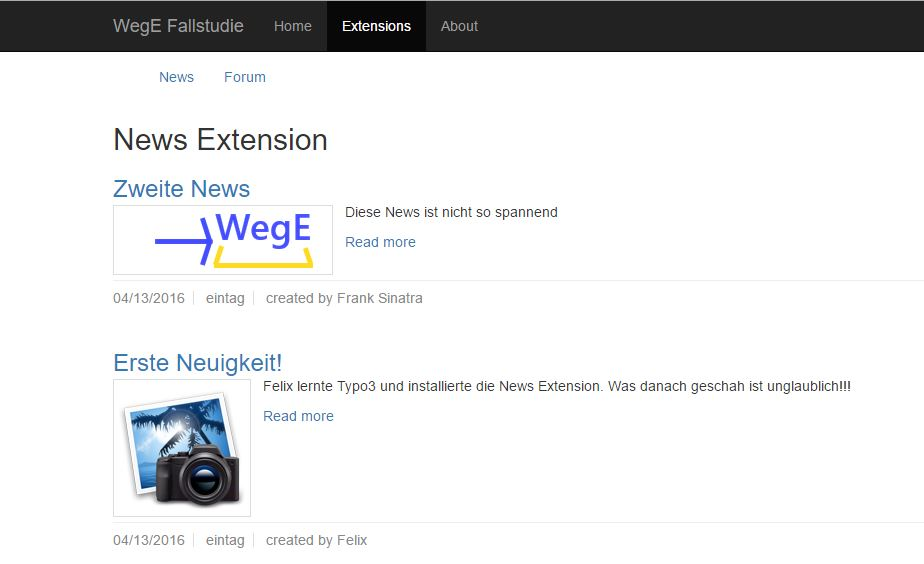
\includegraphics[width=0.75\linewidth]{abb/newsextension.jpg}
\caption[News Extension]{Das Ergebnis der news Extension}
\label{fig:newsextension}
\end{figure}


\subsection{Evaluation}
Die \texttt{news} Extension bietet alle Funktionalit�ten, die man f�r die Anzeige von News jemals brauchen wird. Die Implementation geht schnell, wenn auch nicht unbedingt beim ersten Mal. Alles in Allem ist diese Extension eine exzellente Wahl.

\section{Forum}

\subsection{M�glichkeiten}

\subsection{Implementation}

\subsection{Evaluation}


\section{Anbindung an bestehende Systeme wie Opus}

\subsection{M�glichkeiten}

\subsection{Implementation}

\subsection{Evaluation}


\section{Teilen von wissenschaftlichen Arbeiten}

\subsection{M�glichkeiten}

\subsection{Implementation}

\subsection{Evaluation}

\section{Weitere n�tzliche Extensions}

\begin{itemize}

\item RealURL - h�sche urls
\item Powermail - form
\item MetaSEO Enhancements - page seo
\item Yag - Fotogalerie
\item Grid Elements - Spalten f�r den WYSIWYG
\item Mask - Eigene Contentelemente machen

\end{itemize}


\section{Wartung}
